\chapter{Considerações Finais}
	\section{Conclusões do Projeto de Formatura}
	\section{Perspectivas de Continuidade}
	Mesmo com a relativa complexidade do projeto desenvolvido nessa monografia, diversos pontos se mantém abertos no \textit{backlog}, provenientes da metodologia descrita em capítulos passados desse documento. Com a completude do MVP, é esperado que esses pontos sejam atacados no ano de 2019, idealmente com os integrantes da concepção participando do desenvolvimento de forma direta ou indireta (consultiva). Quanto às perspectivas de manutenção, melhorias e desenvolvimento de novas \textit{features} do \textit{Formicarium}, alguns modos de trabalho se mostram possíveis:
	\begin{enumerate}
	    \item \textit{Squad} (com 3 a 5 engenheiros) totalmente alocados para execução destas atividades.
	    \item \textit{Pack} (2 a 5 engenheiros) dentro de um \textit{squad} horizontal (que dá suporte aos outros engenheiros, como \textit{devops}, \textit{engineering productivity}, \textit{etc.}) alocados para a execução dessas atividades.
	    \item \textit{Task Force} (pelo menos dois engenheiros), participantes de quaisquer \textit{squads}, que desenvolvem \textit{features} no tempo livre das responsabilidades e priorizações de seus \textit{squads}.
	    \item Suspensão do projeto por tempo determinado ou indeterminado.
	\end{enumerate}
	
	Supondo que a alocação de pessoas para trabalhar no projeto se mostre interessante e esteja alinhada aos interesses da empresa (o último item da lista acima não seja o escolhido), levantamos com os \textit{stakeholders} os seguintes requisitos, que agregam algum tipo de valor à experiência do usuário final (por agora não mensurados, porém com ganhos qualitativos evidentes) ou por ajudarem a manutenção e testabilidade da \textit{code base}. A descrição de alto nível dessas tarefas está a seguir:
	
	\begin{description}
  \item[Cache compartilhado de dependências]
  \hfill \\As dependência de \textit{Maven} dos microsserviços \textit{Clojure} desenvolvidos no Nubank são salvas na pasta \url{~\.m2} do contêiner alocado para execução do processo. Os testes empíricos realizados com manipulação de \textit{Devspaces} mostraram um pequeno incômodo: Quando o serviço é executado pela primeira vez no \textit{cluster}, nenhuma dependência existe no repositório mencionado. Por conta disso, toda a árvore de dependências tem que ser obtida do repositório remoto do \textit{Maven}. Este processo pode levar até 20 minutos para um serviço usual do Nubank, apesar de sincronizações futuras (utilizando o mecanismo de \textit{FileSync}) serem praticamente instantâneas.\\
  Estes 20 minutos de espera da primeira vez podem gerar frustrações, e é desejado uma experiência mais ágil de interação e desenvolvimento dos microsserviços. Para resolver este problema, uma possível solução é fazer uma espécie de \textit{cache} compartilhado dos pacotes \textit{Maven}. Como todos os \textit{Devspaces} são executados em um mesmo ambiente da empresa (a saber, \textit{stack} de teste), é possível criar um volume (utilizando o AWS \textit{Elastic Block Storage}) compartilhado por todos os \textit{Devspaces} onde a pasta \url{~\.m2} será montada. A montagem deste volume compartilhado dentro do contêiner obviamente é mais rápido do que o \textit{download} de todas as dependências através da \textit{internet}, tornando o \textit{deploy} de um serviço novo no \textit{Formicarium} muito mais rápido.
  \item[Kafka Facade Service]   
  \hfill \\Um outro projeto de melhoria possível seria a criação de um \textit{Facade} para lidar com a \textit{API} de kafka via linha de comando ou \textit{UI}. A primeira versão do \textit{Formicarium}, descrita nessa monografia suporta apenas chamadas \textit{HTTP} como forma de iniciar um fluxo que envolve vários microsserviços. No entanto, uma coisa muito corrente que se deseja avaliar enquanto se lida com microsserviços é a maneira como o mesmo "altera o mundo" (eg, mudanças de estado, chamadas de API, mensagens enviadas, \textit{logs} reportados, etc) a partir do consumo de uma mensagem \textit{Kafka}. O \textit{Formicarium} provê facilmente para o desenvolvedor apenas a interação via \textit{HTTP}. Engenheiros mais versados em infraestrutura de \textit{Kafka} poderão lidar com o consumo de mensagens para iniciar um fluxo no \textit{Devspace} usando a \textit{API} nativa do \textit{Kafka}, mas este é um processo cansativo e propenso a erros.\\
  Para lidar com isso, pensamos na criação de um serviço para servir como \textit{Facade} para a \textit{API} nativa do \textit{Kafka}, expondo via \textit{HTTP} uma simplificação/agregação das funcionalidades expostas nos binários de implementação de \textit{Kafka}. Com o suporte nativo dado pelo \textit{Formicarium} para \textit{HTTP} ficaria simples de portar essas chamadas ao \textit{Facade} na \textit{UI} e na \textit{CLI}. Vale apontar que esse \textit{Facade} tem valor de negócio para a empresa independentemente do \textit{Formicarium}, pois facilita a interação direta dos desenvolvedores para uma das entradas de dados de seus microsserviços.
  \item[Arquivo de descrição de fluxo de negócio]
  \hfill \\Na implementação corrente o \textit{Formicarium} não provê uma maneira de fazer \textit{deploy} simultâneo de diversos serviços "de uma vez". Isso quer dizer que, para testar a interação de diversos microsserviços, hoje o usuário do \textit{Formicarium} terá que saber a priori, todos os serviços envolvidos no fluxo e subir todos, um a um. Um projeto possível de extensão do \textit{Formicarium} com bastante valor seria criar uma funcionalidade que permitisse a descrição de \textbf{Fluxos de Negócio} (conjunção de vários serviços), descritos num arquivo com formatação específica (podendo ser \textit{yaml}, \textit{xml}, \textit{json}, etc).
  \\Só isso já economizaria bastante tempo do desenvolvedor, que daria um único comando para fazer \textit{deploy} de diversos serviços e não precisaria conhecer todos, a priori.
  \\Com isso funcionando, uma \textit{feature} de exportagem e compartilhamento de fluxos, compostos por um conjunto de serviços e versões específicas dos mesmos seria possível, dando ainda maior poder e autonomia para os engenheiros pensarem em modificações e impactos das mesmas na lógica de negócio que envolve mais de um serviço. 
  \item[Flamegraph]
  \hfill \\Flamegraph é um tipo de gráfico bastante interessante para representação temporal de um fluxo de eventos (opcionalmente independentes entre si). Ele demonstra o tempo gasto processando cada evento, exatamente na ordem em que os eventos foram processados. A figura \ref{fig:flamegraph-example} mostra um exemplo de \textit{flamegraph}.\\
	Hoje o \textit{Formicarium} provê apenas uma visualização de grafo de acontecimento dos eventos, que é muito bom para ver a estrutura de chamadas e os serviços envolvidos, mas deixa um pouco a desejar quando o usuário quer ter um detalhamento mais granular nos tempos de processamento envolvidos. Nesse contexto, implementar uma visualização de \textit{Flamegraph} para os eventos se mostraria vantajoso pois estenderia as possibilidades de \textit{debugging} de um conjunto de eventos providas pelo \textit{Formicarium}.
	\begin{figure}[htb]
		\caption{\label{fig:flamegraph-example}Exemplo de flamegraph}
		\begin{center}
		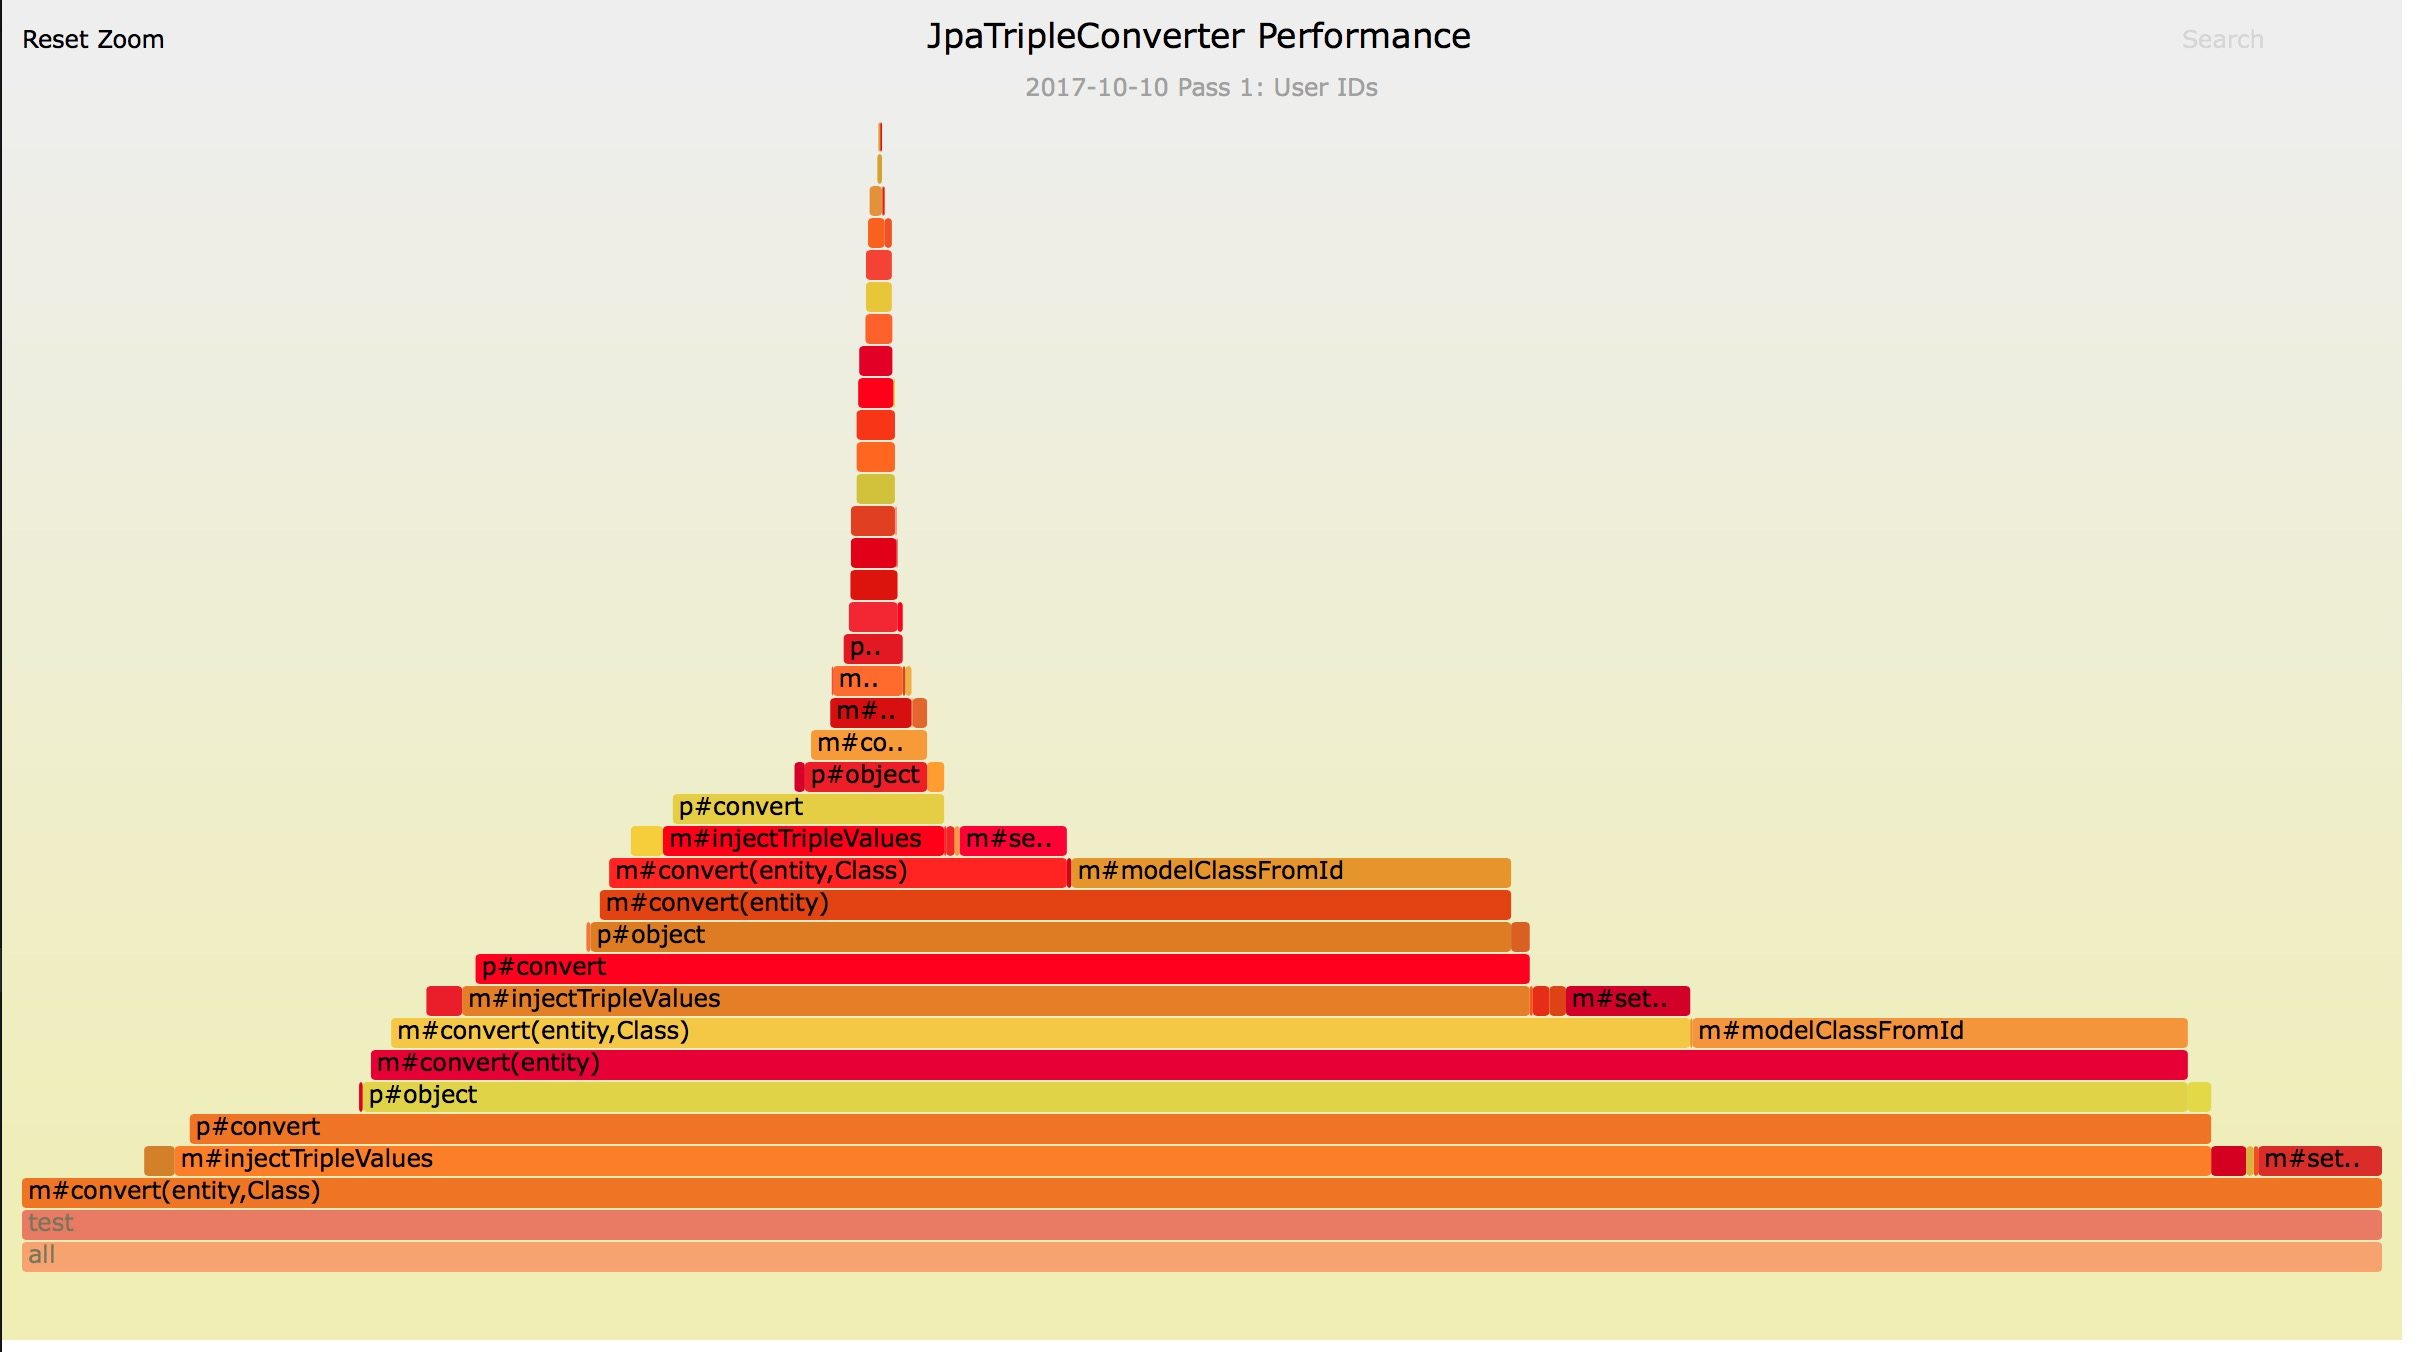
\includegraphics[width=\textwidth,keepaspectratio]{pictures/flame-graph-example.jpg}
		\end{center}
		\legend{Fonte: https://rickosborne.org/blog/tag/flame-graph/}
	\end{figure}
\end{description}
